\documentclass[12pt]{article}
\usepackage[a4paper]{geometry}
\usepackage[utf8]{inputenc}
\usepackage[ngerman]{babel}
\usepackage[T1]{fontenc}
\usepackage{newpxtext,newpxmath}
\usepackage[hidelinks]{hyperref}
\usepackage{amsmath}
\usepackage{mathtools}
\usepackage[style=authoryear-ibid,backend=biber]{biblatex}
\usepackage{csquotes}
\usepackage{fancyhdr}
\usepackage{microtype}

\linespread{1.5}
\parindent 0ex
\bibliography{bibliography.bib}

\pagestyle{fancy}
\fancyhead{}
\fancyfoot{}
\fancyhead[L]{\MakeUppercase{}}
\fancyhead[R]{\MakeUppercase{\leftmark}}
\fancyfoot[C]{\thepage}
\setlength{\headheight}{15pt}

\begin{document}

\begin{titlepage}
  \begin{center}
    \vspace*{1cm}
    \large{\textbf{HTL Rankweil}}\\
    \large{\textbf{5AHEL 2020/21}}
    \vfill
    \line(1,0){400}\\[1mm]
    \huge{\textbf{DIPLOMARBEIT}}\\[3mm]
    \large{\textbf{Advanced Parking Monitoring (APM)}}\\[1mm]
    \line(1,0){400}\\
    \vfill
    Philipp Kraft, Dennis Köb und Samuel Bleiner\\[3mm]
    Dipl.-Ing. Christoph Stüttler \\[6mm]
    \today, Rankweil
  \end{center}
\end{titlepage}

%\pagebreak
%\thispagestyle{empty}
%\hspace{0pt}
%\vfill
%\begin{figure}[h]
%  \centering
%  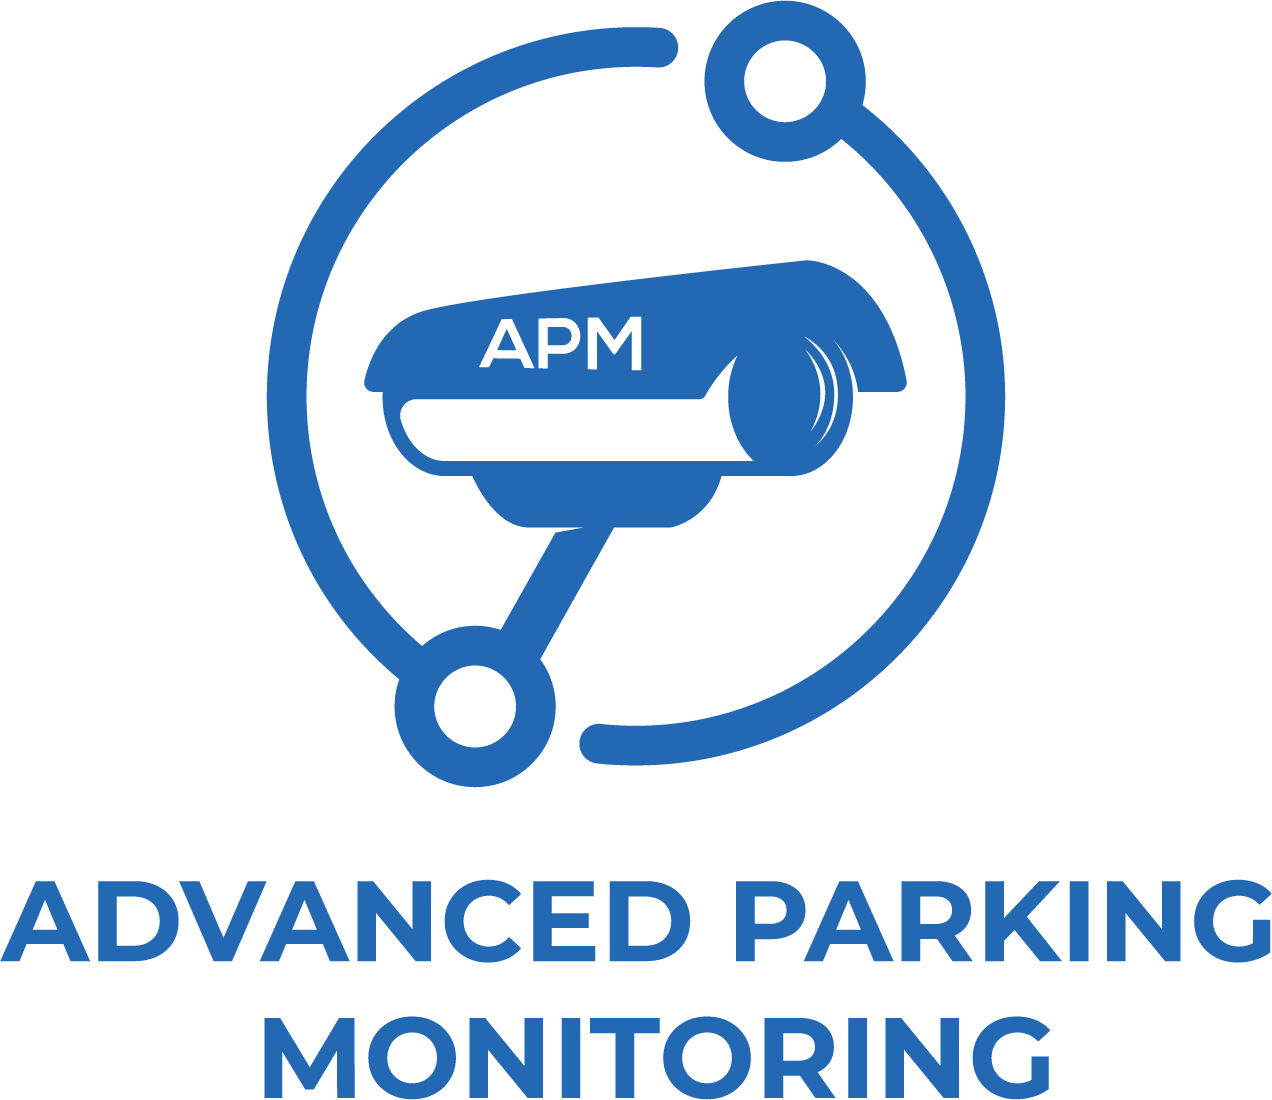
\includegraphics[width=\textwidth]{APM_Logo_Transparent.png}
%  \label{fig:apm_logo}
%\end{figure}
%\vfill
%\hspace{0pt}


\pagenumbering{roman}
\section*{Eidesstattliche Erklärung}
\addcontentsline{toc}{section}{Eidesstattliche Erklärung}
Ich erkläre an Eides statt, dass ich die vorliegende Diplomarbeit selbständig und ohne fremde Hilfe verfasst, andere als die angegebenen Quellen und Hilfsmittel nicht benutzt und die den benutzten Quellen wörtlich und inhaltlich entnommenen Stellen als solche erkenntlich gemacht habe.

\vspace*{1cm}
Rankweil, \today

\vspace*{2cm}


\begin{center}
\begin{tabular}{cp{2em}c} 
  \hspace{6cm} \\\cline{1-1}\cline{3-3}
  \\[-3mm]
  {\footnotesize Philipp Kraft}
\end{tabular}

\vspace*{1cm}

\begin{tabular}{cp{2em}c} 
  \hspace{6cm} \\\cline{1-1}\cline{3-3}
  \\[-3mm]
  {\footnotesize Dennis Köb}
\end{tabular}

\vspace*{1cm}

\begin{tabular}{cp{2em}c} 
  \hspace{6cm} \\\cline{1-1}\cline{3-3}
  \\[-3mm]
  {\footnotesize Samuel Bleiner}
\end{tabular}

\end{center}

\cleardoublepage


\pagebreak

\section*{Kurzfassung}
\addcontentsline{toc}{section}{Kurzfassung}
\lipsum[1-2]
\pagebreak

\section*{Abstract}
\addcontentsline{toc}{section}{Abstract}
\lipsum[1-2]
\pagebreak

\section*{Vorwort}
\addcontentsline{toc}{section}{Vorwort}
In den Jahren unserer Ausbildungszeit ist uns immer wieder aufgefallen, dass
öffentliche gebührenpflichtige Parkplätze kaum moderne technische Innovationen für Zutritt und Abrechnung nutzen.
Daraufhin haben wir uns durch zusätzliche Anregung von unserem
Betreuungslehrer Dipl.-Ing. Christoph Stüttler dazu entschieden, diese Thematik
für unsere Diplomarbeit heranzuziehen.\\

Diese Diplomarbeit soll aufzeigen, wie eine modernes System zur
Parkplatzverwaltung aussehen könnte. Es werden in dieser Arbeit verschiedene
Themenbereiche wie Webinterfaces, künstliche Intelligenz und Mikrocontroller
behandelt.
\pagebreak

\section*{Danksagung}
\addcontentsline{toc}{section}{Danksagung}
Mit dieser Seite wollen wir uns bei allen Personen bedanken die uns zum Erfolg unserer Diplomarbeit geführt haben. 
Wir bedanken uns ausdrücklich bei unserem Betreuungslehrer Dipl.-Ing. Christoph Stüttler für seine fachliche Expertise sowie für alle kreativen Ratschläge während des 
gesamten Betreuungszeitraumes. \\

Unser hauptsächlicher Dank gilt der Firma Omicron für die finanzielle Unterstützung ohne welche die Diplomarbeit in dieser Form nicht existieren würde.\\

Ein herzliches Dankeschön geht an unsere Eltern für ihre Hilfe und für ihren Beistand während unserer gesamten Ausbildungszeit.
\pagebreak
\pagenumbering{arabic}

\tableofcontents
\pagebreak

\setcounter{page}{1}
\section{Einleitung}
\cite{Quille2019} is a citation from an academic journal.\\\
\cite{Quille:Gender} is a citation from a conference proceeding.
\pagebreak

\section{Projektantrag}
\subsection{Name der Arbeit}
APM - Advanced Parking Monitoring

\subsection{Abgabetermin}
Die Abgabe von diesem Antrag ist am ??.10.2020 vorgesehen.

\subsection{Schule und Abteilung}
Höhere Technische Bundeslehr- und Versuchsanstalt Rankweil\\
Negrellistraße 50, A-6830 Rankweil\\
Schulleiterin: Mag. Zeiner-Mohr Judith\\

Elektronik und Technische Informatik\\
Abeitlungsvorstand: Dipl.-Ing. Moosbrugger Leopold

\subsection{Ausgangslage}
Die Parkplatzsuche in Städten verursacht beträchtliche Zeitverluste und eine untragbare Umweltbelastung. Das zu entwickelnde System verfügt über einen Schwenk-/Neigekopf mit aufmontiertem Laserabstandssensor. Es scannt Parkplatz für Parkplatz und prüft, ob er mit einem Fahrzeug besetzt ist oder nicht. Die Daten werden per WLAN an eine Zentralstation gesendet. Die Zentralstation sendet die Anzahl der freien Parkplätze an ein oder mehrere Anzeigeeinheiten. Eine komfortable Eingabemöglichkeit der Parkplatzpositionen ist vorzusehen.

\subsection{Individuelle Themenstellungen}
Für eine ausführliche Individuelle Themenstellung ist es zu früh, daher ist diese nur unspezifisch angeführt.

\begin{table}[htb]
  \begin{tabular}{|l|l|l|}
    \hline
    \textbf{Vor- und Nachname} & \textbf{Individuelle Themenstellung} & \textbf{Klasse} \\ \hline
    Philipp Kraft              & Projektmanagment/Software            & 5AHEL           \\ \hline
    Dennis Köb                 & Hardware                             & 5AHEL           \\ \hline
    Samuel Brugger             & Software/Hardware                    & 5AHEL           \\ \hline
  \end{tabular}
\end{table}

\subsection{Beteiligte Betreuer/innen}
Dipl.-Ing. Stüttler Christoph

\subsection{Beteiligte Kooperationspartner/innen}
Derzeit sind keine Kooperationspartner/innen vorhanden.

\subsection{Rechtliche Regelung}
Die Rechtliche Regelung erfolgt durch die HTL Rankweil.

\subsection{Zielsetzung}
Es ist ein System zu entwerfen, mit dem es möglich ist fesgelegte Parkplätze automatisch zu scannen und somit zu erkennen ob dieser Parkplatz besetzt ist.

\subsection{Kurzfassung/Abstract}
Es ist ein System zu entwerfen, welches es ermöglicht öffentliche Parkplätze zu überwachen und verwalten. Das System ist dabei modular und kostengünstig.

\subsection{Typ der Arbeit}
§ 7 Abs. 1 PrüfOrd. BHS, BA definiert:

„Die Diplomarbeit an höheren Schulen (§ 2 Abs. 4 Z 1 lit. a)
besteht nach Maßgabe des 4. Abschnittes aus einer auf vorwissenschaftlichem Niveau zu erstellenden
schriftlichen Arbeit (bei entsprechender Aufgabenstellung auch unter Einbeziehung praktischer und/oder
grafischer Arbeitsformen) mit Diplomcharakter über ein Thema gemäß § 3 sowie deren Präsentation und
Diskussion.
\pagebreak

\section{Projektvorstudie}
\input{chapters/9_projektvorstudie.tex}
\pagebreak

\section{Hauptteil}
\input{chapters/10_hauptteil.tex}
\pagebreak

\section{Zusammenfassung und Ausblick}
\begin{table}[h]
  \centering
  \resizebox{\textwidth}{!}{%
  \begin{tabular}{@{}cclccc@{}}
  \toprule
  \textbf{Datum} & \textbf{Typ}     & \multicolumn{1}{c}{\textbf{Beschreibung}}              & \textbf{PK}   & \textbf{DK}          & \textbf{SB}          \\ \midrule
  2020-07-13     & Dokumentation    & Erstellung der Thesis mit LaTeX                        & 6 h           & 0 h                  & 0 h                  \\
  2020-07-15     & Projektmanagment & Erstellung der Grundlegenden   Arbeitspaketen          & 2 h           & 0 h                  & 0 h                  \\
  2020-08-15 &
    Entwicklung &
    \begin{tabular}[c]{@{}l@{}}Implementierung Grundlegender   Benutzeroberfläche (Sidebar, Navbar)\\      Implementierung Login/Register System\#\\      Implementierung User Übersicht\end{tabular} &
    6 h &
    0 h &
    0 h \\
  2020-08-21     & Projektmanagment & Erstellung Übersicht von   Zeitaufwendungen und Kosten & 1h            & 0 h                  & 0 h                  \\
  2020-08-21     & Dokumentation    & Überarbeitung der Thesis                               & 1 h           & \multicolumn{1}{l}{} & \multicolumn{1}{l}{} \\
                 &                  &                                                        &               &                      &                      \\ \midrule
  \multicolumn{3}{c}{\multirow{2}{*}{\textbf{Gesamtaufwand}}}                                & \textbf{15 h} & \textbf{0 h}         & \textbf{0 h}         \\ \cmidrule(l){4-6} 
  \multicolumn{3}{c}{}                                                                       & \multicolumn{3}{l}{\textbf{15 h}}                           \\ \bottomrule
  \end{tabular}%
  }
  \caption{Zeitaufwendungen}
  \label{tab:zeitaufwendungen}
  \end{table}
\pagebreak

\section{Begleitprotokoll}
\input{chapters/12_begleitprotokoll.tex}
\pagebreak

\section{Anhang}
\begin{listing}[H]
  \begin{minted}{bash}
    mv phpMyAdmin-5.0.4-all-languages /usr/share/phpmyadmin/usr/share/ phpmyadmin/usr/share/phpmyadmin
    mkdir -p /var/lib/phpmyadmin/tmp
    chown -R www-data:www-data /var/lib/phpmyadmin
    mkdir /etc/phpmyadmin/
  \end{minted}
  \caption{Example of a listing}
  \label{lst:example}
\end{listing}

\pagebreak

\listoffigures
\addcontentsline{toc}{section}{Abbildungsverzeichnis}
\pagebreak

\listoftables
\addcontentsline{toc}{section}{Tabellenverzeichnis}
\pagebreak

\section*{Abkürzungsverzeichnis}
\addcontentsline{toc}{section}{Abkürzungsverzeichnis}
\pagebreak

\printbibliography[title=Literaturverzeichnis]
\addcontentsline{toc}{section}{Literaturverzeichnis}
\pagebreak

\end{document}
